\documentclass[11pt]{article}
%%% full alphabets of different styles %%%

% bf series
\def\bfA{\mathbf{A}}
\def\bfB{\mathbf{B}}
\def\bfC{\mathbf{C}}
\def\bfD{\mathbf{D}}
\def\bfE{\mathbf{E}}
\def\bfF{\mathbf{F}}
\def\bfG{\mathbf{G}}
\def\bfH{\mathbf{H}}
\def\bfI{\mathbf{I}}
\def\bfJ{\mathbf{J}}
\def\bfK{\mathbf{K}}
\def\bfL{\mathbf{L}}
\def\bfM{\mathbf{M}}
\def\bfN{\mathbf{N}}
\def\bfO{\mathbf{O}}
\def\bfP{\mathbf{P}}
\def\bfQ{\mathbf{Q}}
\def\bfR{\mathbf{R}}
\def\bfS{\mathbf{S}}
\def\bfT{\mathbf{T}}
\def\bfU{\mathbf{U}}
\def\bfV{\mathbf{V}}
\def\bfW{\mathbf{W}}
\def\bfX{\mathbf{X}}
\def\bfY{\mathbf{Y}}
\def\bfZ{\mathbf{Z}}
\def\bfx{\mathbf{x}}
\def\bfmu{\boldsymbol{\mu}}
\def\bfSigma{\mathbf{\Sigma}}

% bb series
\def\bbA{\mathbb{A}}
\def\bbB{\mathbb{B}}
\def\bbC{\mathbb{C}}
\def\bbD{\mathbb{D}}
\def\bbE{\mathbb{E}}
\def\bbF{\mathbb{F}}
\def\bbG{\mathbb{G}}
\def\bbH{\mathbb{H}}
\def\bbI{\mathbb{I}}
\def\bbJ{\mathbb{J}}
\def\bbK{\mathbb{K}}
\def\bbL{\mathbb{L}}
\def\bbM{\mathbb{M}}
\def\bbN{\mathbb{N}}
\def\bbO{\mathbb{O}}
\def\bbP{\mathbb{P}}
\def\bbQ{\mathbb{Q}}
\def\bbR{\mathbb{R}}
\def\bbS{\mathbb{S}}
\def\bbT{\mathbb{T}}
\def\bbU{\mathbb{U}}
\def\bbV{\mathbb{V}}
\def\bbW{\mathbb{W}}
\def\bbX{\mathbb{X}}
\def\bbY{\mathbb{Y}}
\def\bbZ{\mathbb{Z}}

% cal series
\def\calA{\mathcal{A}}
\def\calB{\mathcal{B}}
\def\calC{\mathcal{C}}
\def\calD{\mathcal{D}}
\def\calE{\mathcal{E}}
\def\calF{\mathcal{F}}
\def\calG{\mathcal{G}}
\def\calH{\mathcal{H}}
\def\calI{\mathcal{I}}
\def\calJ{\mathcal{J}}
\def\calK{\mathcal{K}}
\def\calL{\mathcal{L}}
\def\calM{\mathcal{M}}
\def\calN{\mathcal{N}}
\def\calO{\mathcal{O}}
\def\calP{\mathcal{P}}
\def\calQ{\mathcal{Q}}
\def\calR{\mathcal{R}}
\def\calS{\mathcal{S}}
\def\calT{\mathcal{T}}
\def\calU{\mathcal{U}}
\def\calV{\mathcal{V}}
\def\calW{\mathcal{W}}
\def\calX{\mathcal{X}}
\def\calY{\mathcal{Y}}
\def\calZ{\mathcal{Z}}
%%% custom notation %%%

% vector calculus + partial derivatives 
\def\del{{\partial}}
\newcommand{\deriv}[2][]{\frac{d^{#1}}{d{#2}^{#1}}}
\newcommand{\derivP}[2][]{\frac{\del^{#1}}{\del{#2}^{#1}}}

% linear algebra / matrix notation
\newcommand{\iden}[1]{\mathbb{I}_{{#1} \times {#1}}} % n-by-n identity matrix 
\newcommand{\tpose}[1]{{#1}^{\top}} % matrix transpose

% indicator function
\def\1{{\mathbf 1}}
\newcommand{\indic}[1]{\1_{[#1]}}

% statistics terminology
\newcommand{\expec}[2][]{\bbE_{#1}[#2]} 
\newcommand{\prob}[2][]{\bbP_{#1}(#2)}
\newcommand{\var}[2][]{\text{Var}_{#1}[#2]}
\newcommand{\bias}[1]{\textbf{bias}(#1)}
\newcommand{\stderror}[1]{\textbf{se}(#1)}
\newcommand{\MSE}[1]{\text{MSE}(#1)}
\def\simiid{\sim_{\mbox{\tiny \textrm{iid}}}} %sampled i.i.d

% miscellaneous 
\def\fstar{f^{*}}
\usepackage{graphicx, amssymb, amsmath, amsthm, amsfonts, mathrsfs}
\usepackage{multirow, makeidx}
\usepackage{mathtools}
\usepackage{enumerate, enumitem}
\usepackage{pifont}

\usepackage[ruled, linesnumbered]{algorithm2e}
\SetKwRepeat{Repeat}{repeat}{until} 

\usepackage{multicol}
\setlength{\columnsep}{40pt}

\usepackage{titlesec}
\titleformat{\section}
  {\normalfont\Large\bfseries}
  {}
  {0pt}
  {}
\titleformat{\subsection}
  {\normalfont\large\bfseries}
  {}
  {0pt}
  {}

\usepackage{geometry}
\geometry{
    letterpaper,
    left = 0.75in,
    right = 0.75in,
    top = 1.0in,
    bottom = 1.0in    
}
\usepackage{parskip}
\usepackage{scalefnt}
\usepackage{caption,subcaption}
\usepackage{hyperref}
\hypersetup{
    colorlinks=true,
    linkcolor=cyan,
    filecolor=magenta,      
    urlcolor=blue
}

\pagenumbering{gobble}
\numberwithin{figure}{section}
\renewcommand{\thefigure}{\arabic{section}.\arabic{figure}}
\numberwithin{equation}{section}
\renewcommand{\theequation}{\arabic{section}.\arabic{equation}}

\def\BayesOpt{\texttt{BayesOpt}}
\def\EI{\texttt{EI}}
\def\calGP{\mathcal{GP}}

\newcommand{\bs}[1]{\boldsymbol{#1}}
\def\bsx{\bs{x}}
\def\bsy{\bs{y}}
\def\bsk{\bs{k}}
\def\bsd{\bs{d}}
\def\bell{\bs{\ell}}
\def\xast{\bsx_{*}}
\def\Matern{\textrm{Mat\'{e}rn}}

% \usepackage{xparse}
% \NewDocumentCommand{\xinc}{o}{%
%   \bsx_{\textrm{inc}\IfValueT{#1}{,{#1}}}
% }
% \NewDocumentCommand{\yinc}{o}{%
%   y_{\textrm{inc}\IfValueT{#1}{,{#1}}}
% }

\usepackage{tikz}
\usetikzlibrary {angles,quotes}


\begin{document}

\section{Context}

This document contains mathematical derivations for an altered version of a \BayesOpt{} algorithm in which the dataset only ever has two recorded values, with additional values `thrown out' at each iteration of the algorithm.

Part of the reason for creating this algorithm is to mathematically determine whether the algorithm proposed in \href{https://arxiv.org/abs/2402.02229}{\textit{Vanilla Bayesian Optimization Performs Great in High Dimensions}} is primarily (from a conceptual standpoint) just performing local Bayesian optimization in a high-dimensional space.

\noindent\rule{\textwidth}{0.8pt}

\section{Theoretical Setup}

We want to perform Bayesian Optimization (\BayesOpt) to find the global maximum of an unknown real-valued function $\fstar(\cdot)$ defined on a compact space $\calX \subset \bbR^{D}$. For the sake of simplicity, we will assume that $\calX = [0,1]^{D}$.

To achieve this goal, we use a Gaussian process model $\fstar \sim \calGP\left(\mu_{f}(\cdot), \sigma_{f}^{2}k_{\bell}(\cdot, \cdot)\right)$, where $k_{\bell}(\cdot, \cdot)$ is an RBF (radial basis function) kernel with lengthscale hyperparameter $\bell \in \bbR^{D}$. For now, we fix $\bell = \begin{pmatrix}1 & \cdots & 1\end{pmatrix}^{\top}$.

Unlike traditional \BayesOpt{} algorithms which update the posterior of $\fstar$ after each iteration based on \textbf{all} collected datapoints, we propose a `forgetful' algorithm, in which the dataset only ever contains two observations: the \textit{incumbent} (maximum value observed thus far) and the most-recent non-incumbent.

\section{Assumptions}

In the analysis of this algorithm, we make the following assumptions:

\begin{itemize}[label=\ding{228}]

  \item We can model our unknown function as a Gaussian process of the form $\fstar \sim \calGP\left(\mu_{f}(\cdot), \sigma_{f}^{2}k_{\bell}(\cdot, \cdot)\right)$
  \begin{itemize}[label=\ding{118}]
    \item Furthermore, we assume that $\mu_{f}(\bsx) = 0$ for all $\bsx \in \calX$, and that $\sigma_{f} = 1$ by scaling the function as required.
  \end{itemize}

  \item We assume that $\calX$ is a \textbf{convex} subset of $\bbR^{D}$. 
  \begin{itemize}[label=\ding{118}]
    \item Furthermore, we will assume that $\calX$ is the unit hypercube $[0, 1]^{D}$.
  \end{itemize}

  \item We query \textit{noiseless} observations $y_{i} = \fstar(\bsx_{i})$, i.e. the observation noise parameter $\sigma_{\epsilon}$ is 0. 

  \item $k_{\bell}(\cdot, \cdot)$ is a radial covariance kernel (stationary kernel which depends only on distance) which is affected by the lengthscale hyperparameter $\bell$.
  \begin{itemize}[label=\ding{118}]
    \item In particular, we have some distance metric $d_{\bell}(\cdot, \cdot)$ where $k_{\bell}(a, b)$ depends only on $d_{\bell}(a,b)$.
  \end{itemize}

  \item The next queried point in each iteration of the algorithm is chosen by maximizing the expected improvement (\EI{}) with respect to the current dataset. 

  \item At each iteration $t$ of the algorithm, $y_{0} \ge y_{1}$. This can be done without loss of generality by relabelling as needed.
\end{itemize}

\newpage

\section{Maximizing \EI}

Let $\calD_{t} = (\mathbf{X}, \mathbf{y})$ be the dataset of two observations at time $t$. For ease of notation, we let $\bsk_{01} = k_{\bell}(\bsx_{0}, \bsx_{1})$, $\bsk_{0*} = k_{\bell}(\xast, \bsx_{0})$, and $\bsk_{1*} = k_{\bell}(\xast, \bsx_{1})$. Note that these are all scalar values. Under the assumptions outlined above, for all $\xast \in \calX$, we have the following:
\begin{align*}
\expec{f(\xast) \mid \mathbf{X}, \mathbf{y}} &= \mu_{f}(\xast) + k_{\bell}(\xast, \mathbf{X})k_{\bell}(\mathbf{X}, \mathbf{X})^{-1}(\mathbf{y} - \mu_{f}(\mathbf{X}))\\
&= 0 + \begin{pmatrix}\bsk_{0*} & \bsk_{1*}\end{pmatrix}\begin{pmatrix}1 & \bsk_{01}\\ \bsk_{01} & 1\end{pmatrix}^{-1}\begin{pmatrix}\bsy_0 - 0\\ \bsy_{1} - 0\end{pmatrix}\\
&= \frac{1}{1 - \bsk_{01}^2}\begin{pmatrix}\bsk_{0*} & \bsk_{1*}\end{pmatrix}\begin{pmatrix}1 & -\bsk_{01}\\ -\bsk_{01} & 1\end{pmatrix}\begin{pmatrix}\bsy_0\\ \bsy_{1}\end{pmatrix}\\
&= \frac{1}{1 - \bsk_{01}^2}\left[\bsk_{0*}\left(\bsy_{0} - \bsk_{01}\bsy_{1}\right) + \bsk_{1*}\left(\bsy_{1} - \bsk_{01}\bsy_{0}\right)\right]\\
\var{f(\xast) \mid \mathbf{X}, \mathbf{y}} &= \sigma_{f}^{2} - k_{\bell}(\xast, \mathbf{X})k_{\bell}(\mathbf{X}, \mathbf{X})^{-1}k_{\bell}(\mathbf{X}, \xast)\\
&= 1 - \begin{pmatrix}\bsk_{0*} & \bsk_{1*}\end{pmatrix}\begin{pmatrix}1 & \bsk_{01}\\ \bsk_{01} & 1\end{pmatrix}^{-1}\begin{pmatrix}\bsk_{0*}\\ \bsk_{1*}\end{pmatrix}\\
&= 1 - \frac{1}{1 - \bsk_{01}^{2}}\begin{pmatrix}\bsk_{0*} & \bsk_{1*}\end{pmatrix}\begin{pmatrix}1 & -\bsk_{01}\\ -\bsk_{01} & 1\end{pmatrix}\begin{pmatrix}\bsk_{0*}\\ \bsk_{1*}\end{pmatrix}\\
&= 1 - \frac{1}{1 - \bsk_{01}^{2}}\left[\bsk_{0*}^{2} - 2\bsk_{01}\bsk_{0*}\bsk_{1*} + \bsk_{1*}^{2}\right]\\
&= \frac{1}{1 - \bsk_{01}^{2}}\left[1 - \left(\bsk_{01}^{2} + \bsk_{0*}^{2} + \bsk_{1*}^{2}\right) + 2\bsk_{01}\bsk_{0*}\bsk_{1*}\right]\\
\end{align*}
Unfortunately, even with only 2 observations, it is difficult to get a `nice' closed-form expression for $\var{f(\xast) \mid \mathbf{X}, \mathbf{y}}$, and computing the square root of this value is no better. 

For $\xast \in \calX$, define $\mu_{\textrm{post}}(\xast) = \expec{f(\xast) \mid \mathbf{X}, \mathbf{y}}$, and $\sigma_{\textrm{post}}(\xast) = \sqrt{\var{f(\xast) \mid \mathbf{X}, \mathbf{y}}}$.

By definition, $\EI(\xast \mid \mathbf{X}, \mathbf{y}) = \expec{\max\left(0, f(\xast) - \bsy_{0}\right) \mid \mathbf{X}, \mathbf{y}}$. We know that this can be simplified to 
\begin{equation*}
\EI(\xast \mid \mathbf{X}, \mathbf{y}) = \left(\mu_{\textrm{post}}(\xast) - \bsy_{0}\right)\Phi\left(\frac{\mu_{\textrm{post}}(\xast) - \bsy_{0}}{\sigma_{\textrm{post}}(\xast)}\right) + \sigma_{\textrm{post}}(\xast)\phi\left(\frac{\mu_{\textrm{post}}(\xast) - \bsy_{0}}{\sigma_{\textrm{post}}(\xast)}\right)
\end{equation*}
\noindent\rule{\textwidth}{0.8pt}

From above, we have that $\mu_{\textrm{post}}(\xast) = \frac{1}{1 - \bsk_{01}^2}\left[\bsk_{0*}\left(\bsy_{0} - \bsk_{01}\bsy_{1}\right) + \bsk_{1*}\left(\bsy_{1} - \bsk_{01}\bsy_{0}\right)\right]$, and that $\sigma_{\textrm{post}}(\xast) = \sqrt{\frac{1 - \left(\bsk_{01}^{2} + \bsk_{0*}^{2} + \bsk_{1*}^{2}\right) + 2\bsk_{01}\bsk_{0*}\bsk_{1*}}{1 - \bsk_{01}^{2}}}$. Note that both $\mu_{\textrm{post}}$ and $\sigma_{\textrm{post}}$ depend only on $\bsk_{0*}$ and $\bsk_{1*}$, not on the value of $\xast$ itself. For simplicity, we can treat these as functions of $\bsk_{0*}$ and $\bsk_{1*}$, as opposed to treating them as univariate functions of $\xast$. 

Based on this, we can also write \EI{} as a function of $\bsk_{0*}$ and $\bsk_{1*}$, i.e. $$\EI(\bsk_{0*}, \bsk_{1*}) = \left(\mu_{\textrm{post}}(\bsk_{0*}, \bsk_{1*}) - \bsy_{0}\right)\Phi\left(\frac{\mu_{\textrm{post}}(\bsk_{0*}, \bsk_{1*}) - \bsy_{0}}{\sigma_{\textrm{post}}(\bsk_{0*}, \bsk_{1*})}\right) + \sigma_{\textrm{post}}(\bsk_{0*}, \bsk_{1*})\phi\left(\frac{\mu_{\textrm{post}}(\bsk_{0*}, \bsk_{1*}) - \bsy_{0}}{\sigma_{\textrm{post}}(\bsk_{0*}, \bsk_{1*})}\right)$$ and we can maximize \EI{} with respect to the kernels $\bsk_{0*}, \bsk_{1*}$.

{\footnotesize
\begin{align*}
\frac{\partial \EI}{\partial \bsk_{0*}} &= \left(\frac{\partial \EI}{\partial \mu_{\textrm{post}}}\right)\left(\frac{\partial \mu_{\textrm{post}}}{\partial \bsk_{0*}}\right) + \left(\frac{\partial \EI}{\partial \sigma_{\textrm{post}}}\right)\left(\frac{\partial \sigma_{\textrm{post}}}{\partial \bsk_{0*}}\right) \tag{Multivariate Chain Rule}\\
&= \left[\Phi\left(\frac{\mu_{\textrm{post}} - \bsy_{0}}{\sigma_{\textrm{post}}}\right) + \left(\frac{\mu_{\textrm{post}} - \bsy_{0}}{\sigma_{\textrm{post}}}\right)\phi\left(\frac{\mu_{\textrm{post}} - \bsy_{0}}{\sigma_{\textrm{post}}}\right) + \phi'\left(\frac{\mu_{\textrm{post}} - \bsy_{0}}{\sigma_{\textrm{post}}}\right)\right]\left(\frac{\bsy_{0} - \bsk_{01}\bsy_{1}}{1 - \bsk_{01}^2}\right) +\\
&\quad \left[\left(1 - \left(\frac{\mu_{\textrm{post}} - \bsy_{0}}{\sigma_{\textrm{post}}}\right)^{2}\right)\phi\left(\frac{\mu_{\textrm{post}} - \bsy_{0}}{\sigma_{\textrm{post}}}\right) - \left(\frac{\mu_{\textrm{post}} - \bsy_{0}}{\sigma_{\textrm{post}}}\right)\phi'\left(\frac{\mu_{\textrm{post}} - \bsy_{0}}{\sigma_{\textrm{post}}}\right)\right]\left(\frac{\bsk_{01}\bsk_{1*} - \bsk_{0*}}{\left(1 - \bsk_{01}^{2}\right)\sigma_{\textrm{post}}}\right)
\intertext{Substituting $Z(\bsk_{0*}, \bsk_{1*}) = \frac{\mu_{\textrm{post}}(\bsk_{0*}, \bsk_{1*}) - \bsy_{0}}{\sigma_{\textrm{post}}(\bsk_{0*}, \bsk_{1*})}$ yields the following:}
\frac{\partial \EI}{\partial \bsk_{0*}} &= \left[\Phi(Z) + Z\phi(Z) + \phi'(Z)\right]\left(\frac{\bsy_{0} - \bsk_{01}\bsy_{1}}{1 - \bsk_{01}^2}\right) + \left[\left(1 - Z^2\right)\phi(Z) - Z\phi'(Z)\right]\left(\frac{\bsk_{01}\bsk_{1*} - \bsk_{0*}}{\left(1 - \bsk_{01}^{2}\right)\sigma_{\textrm{post}}}\right)
\intertext{Note that $\phi(z) = (2\pi)^{-0.5}\exp(-z^2/2)$. Taking a derivative yields that $\phi'(z) = -z\phi(z)$, or equivalently, $z\phi(z) + \phi'(z) = 0$.}
\frac{\partial \EI}{\partial \bsk_{0*}} &= \Phi\left(Z\right)\left(\frac{\bsy_{0} - \bsk_{01}\bsy_{1}}{1 - \bsk_{01}^2}\right) + \phi\left(Z\right)\left(\frac{\bsk_{01}\bsk_{1*} - \bsk_{0*}}{\left(1 - \bsk_{01}^{2}\right)\sigma_{\textrm{post}}}\right)\\
\frac{\partial \EI}{\partial \bsk_{0*}} &\propto \Phi\left(Z\right)\left(\bsy_{0} - \bsk_{01}\bsy_{1}\right) + \phi\left(Z\right)\left(\frac{\bsk_{01}\bsk_{1*} - \bsk_{0*}}{\sigma_{\textrm{post}}}\right)\tag{Since $\bsk_{01}$ is constant}\\
&= \Phi\left(\frac{\mu_{\textrm{post}} - \bsy_{0}}{\sigma_{\textrm{post}}}\right)\left(\bsy_{0} - \bsk_{01}\bsy_{1}\right) + \phi\left(\frac{\mu_{\textrm{post}} - \bsy_{0}}{\sigma_{\textrm{post}}}\right)\left(\frac{\bsk_{01}\bsk_{1*} - \bsk_{0*}}{\sigma_{\textrm{post}}}\right)\tag{Undoing the substitution}\\
\end{align*}
}%
\vfill{}
{\footnotesize
\begin{align*}
\frac{\partial \EI}{\partial \bsk_{1*}} &= \left(\frac{\partial \EI}{\partial \mu_{\textrm{post}}}\right)\left(\frac{\partial \mu_{\textrm{post}}}{\partial \bsk_{1*}}\right) + \left(\frac{\partial \EI}{\partial \sigma_{\textrm{post}}}\right)\left(\frac{\partial \sigma_{\textrm{post}}}{\partial \bsk_{1*}}\right) \tag{Multivariate Chain Rule}\\
&= \left[\Phi\left(\frac{\mu_{\textrm{post}} - \bsy_{0}}{\sigma_{\textrm{post}}}\right) + \left(\frac{\mu_{\textrm{post}} - \bsy_{0}}{\sigma_{\textrm{post}}}\right)\phi\left(\frac{\mu_{\textrm{post}} - \bsy_{0}}{\sigma_{\textrm{post}}}\right) + \phi'\left(\frac{\mu_{\textrm{post}} - \bsy_{0}}{\sigma_{\textrm{post}}}\right)\right]\left(\frac{\bsy_{1} - \bsk_{01}\bsy_{0}}{1 - \bsk_{01}^2}\right) +\\
&\quad \left[\left(1 - \left(\frac{\mu_{\textrm{post}} - \bsy_{0}}{\sigma_{\textrm{post}}}\right)^{2}\right)\phi\left(\frac{\mu_{\textrm{post}} - \bsy_{0}}{\sigma_{\textrm{post}}}\right) - \left(\frac{\mu_{\textrm{post}} - \bsy_{0}}{\sigma_{\textrm{post}}}\right)\phi'\left(\frac{\mu_{\textrm{post}} - \bsy_{0}}{\sigma_{\textrm{post}}}\right)\right]\left(\frac{\bsk_{01}\bsk_{0*} - \bsk_{1*}}{\left(1 - \bsk_{01}^{2}\right)\sigma_{\textrm{post}}}\right)
\intertext{Substituting $Z(\bsk_{0*}, \bsk_{1*}) = \frac{\mu_{\textrm{post}}(\bsk_{0*}, \bsk_{1*}) - \bsy_{0}}{\sigma_{\textrm{post}}(\bsk_{0*}, \bsk_{1*})}$ yields the following:}
\frac{\partial \EI}{\partial \bsk_{1*}} &= \left[\Phi(Z) + Z\phi(Z) + \phi'(Z)\right]\left(\frac{\bsy_{1} - \bsk_{01}\bsy_{0}}{1 - \bsk_{01}^2}\right) + \left[\left(1 - Z^2\right)\phi(Z) - Z\phi'(Z)\right]\left(\frac{\bsk_{01}\bsk_{0*} - \bsk_{1*}}{\left(1 - \bsk_{01}^{2}\right)\sigma_{\textrm{post}}}\right)
\intertext{Note that $\phi(z) = (2\pi)^{-0.5}\exp(-z^2/2)$. Taking a derivative yields that $\phi'(z) = -z\phi(z)$, or equivalently, $z\phi(z) + \phi'(z) = 0$.}
\frac{\partial \EI}{\partial \bsk_{1*}} &= \Phi\left(Z\right)\left(\frac{\bsy_{1} - \bsk_{01}\bsy_{0}}{1 - \bsk_{01}^2}\right) + \phi\left(Z\right)\left(\frac{\bsk_{01}\bsk_{0*} - \bsk_{1*}}{\left(1 - \bsk_{01}^{2}\right)\sigma_{\textrm{post}}}\right)\\
\frac{\partial \EI}{\partial \bsk_{1*}} &\propto \Phi\left(Z\right)\left(\bsy_{1} - \bsk_{01}\bsy_{0}\right) + \phi\left(Z\right)\left(\frac{\bsk_{01}\bsk_{0*} - \bsk_{1*}}{\sigma_{\textrm{post}}}\right)\tag{Since $\bsk_{01}$ is constant}\\
&= \Phi\left(\frac{\mu_{\textrm{post}} - \bsy_{0}}{\sigma_{\textrm{post}}}\right)\left(\bsy_{1} - \bsk_{01}\bsy_{0}\right) + \phi\left(\frac{\mu_{\textrm{post}} - \bsy_{0}}{\sigma_{\textrm{post}}}\right)\left(\frac{\bsk_{01}\bsk_{0*} - \bsk_{1*}}{\sigma_{\textrm{post}}}\right)\tag{Undoing the substitution}\\
\end{align*}
}%

\newpage 

\section{Conditions for \EI{} Maximization}

To solve the system of equations $\frac{\partial}{\partial \bsk_{0*}}\EI(\bsk_{0*}, \bsk_{1*}) = \frac{\partial}{\partial \bsk_{1*}}\EI(\bsk_{0*}, \bsk_{1*}) = 0$, we need to solve two equations of the form $a\Phi(z) + b\phi(z) = 0$, or equivalently, $\frac{\phi(z)}{\Phi(z)} = -\frac{a}{b}$.

\textbf{Lemma:} For any $c_0 > 0, c_1 > 0$, there exists $z \in \bbR$ such that $c_{0}\Phi(z) - c_{1}\phi(z) = 0$. 

\textbf{Proof of Lemma:} The equation above is equivalent to 

%%% Additional slightly irrelevant notes below %%%
\newpage 

\section{Using the \Matern(1/2) Kernel}

Since $k_{\bell}$ is a radial kernel, it depends only on the distance between points. Let $\bsd_{01}, \bsd_{0*}, \bsd_{1*}$ respectively represent $d_{\bell}(\bsx_{0}, \bsx_{1}), d_{\bell}(\bsx_{0}, \xast), d_{\bell}(\bsx_{1}, \xast)$. 

Applying the Triangle Inequality yields $\bsd_{0*} \le \bsd_{01} + \bsd_{1*}$. Thus, $\exp(-\bsd_{0*}) \ge \exp\left(-\left(\bsd_{01} + \bsd_{1*}\right)\right) = \exp(-\bsd_{01})\exp(-\bsd_{1*})$. Thus, when the kernel $k_{\bell}$ is a \Matern(1/2) kernel, we have that $\bsk_{0*} \ge \bsk_{01}\bsk_{1*}$.
\noindent\rule{\textwidth}{0.8pt}

\newpage

\section{Posterior Variance Revisited}
Above, we demonstrated that for any given $\xast \in \calX$, $\var{f(\xast) \mid \mathbf{X}, \mathbf{y}} = 1 - \frac{1}{1 - \bsk_{01}^{2}}\left[\bsk_{0*}^{2} - 2\bsk_{01}\bsk_{0*}\bsk_{1*} + \bsk_{1*}^{2}\right]$ when the dataset $\calD_{t} = (\mathbf{X}, \mathbf{y})$ contains exactly 2 observations. This expression is difficult to work with.

Note that $0 \le \bsk_{01}, \bsk_{0*}, \bsk_{1*} \le 1$ as these are all `scaled' kernels. Consider a triangle with two sides whose lengths are $\bsk_{0*}$ and $\bsk_{1*}$, as shown in the picture below, and suppose that $\cos(A) = \bsk_{01}$.

\vspace*{1.0cm}
\begin{center}
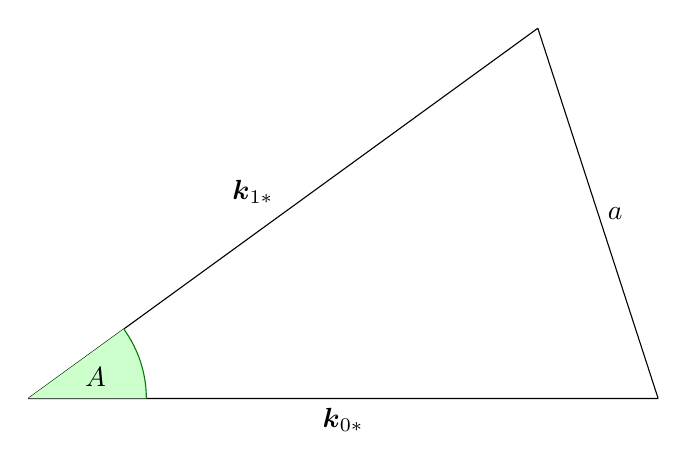
\begin{tikzpicture}[scale=8]
  \coordinate (a) at (0,0);
  \coordinate (b) at (1,0);
  \coordinate (c) at (36:1cm);

  \draw 
    (a) -- (b) node[midway, below]{$\bsk_{0*}$}
    (b) -- (c) node[midway, right]{$a$}
    (c) -- (a) node[midway, above left]{$\bsk_{1*}$} -- cycle;
    \pic[draw=green!50!black, fill=green!20, angle radius=15mm, "$A$"]{angle=b--a--c};
\end{tikzpicture}
\end{center}

By the Law of Cosines, $a^2 = \bsk_{0*}^2 + \bsk_{1*}^{2} - 2\bsk_{0*}\bsk_{1*}\cos(A) = \bsk_{0*}^2 + \bsk_{1*}^{2} - 2\bsk_{0*}\bsk_{1*}\bsk_{01}$. Additionally, $\frac{1}{1 - \bsk_{01}^{2}} = \frac{1}{1 - \cos^{2}(A)} = \frac{1}{\sin^{2}(A)}$. Thus, in terms of the triangle above, $\var{f(\xast) \mid \mathbf{X}, \mathbf{y}} = 1 - \frac{a^2}{\sin^2(A)}$.

Recall that $\bsk_{01}$ is fixed with respect to the choice of $\xast$. Since the angle $A$ depends only on $\bsk_{01}$, this angle is fixed with respect to $\xast$. However, the side lengths of this triangle are dependent on $\xast$, as $\bsk_{0*}$ and $\bsk_{1*}$ are functions of $\xast$. 
% \newpage
% \section{Algorithm Pseudocode}
% \begin{algorithm}
% \caption{General idea for the proposed `forgetful' \BayesOpt{} algorithm}\label{alg:algo-1}
% \SetKwComment{Comment}{/* }{ */}
% \KwData{$\calD_{0} = \left\{\left(\bsx_{0}, y_{0} = \fstar(\bsx_{0})\right), \left(\bsx_{1}, y_{1} = \fstar(\bsx_{1})\right)\right\}$}
% \KwResult{$\arg\max_{x \in \calX}\fstar(x)$}
% \While{$N \neq 0$}{
%   \eIf{$N$ is even}{
%     $X \gets X \times X$\;
%     $N \gets \frac{N}{2}$\;
%   }{\If{$N$ is odd}{
%     $y \gets y \times X$\;
%     $N \gets N - 1$\;
%     }
%   }
% }  
% \end{algorithm}
\end{document}